%----------------------------------------------------------------------------------
% Exemplo do uso da classe tcc.cls. Veja o arquivo .cls
% para mais detalhes e instruções.
%----------------------------------------------------------------------------------
\chapter{\label{chap:chap3}Riscos de Segurança em Contratos Inteligentes}


A presente seção visa fornecer uma análise aprofundada das diversas formas de ataque que podem ser direcionadas a smart contracts, destacando as vulnerabilidades que permeiam esse ecossistema complexo \cite{SMAP}. À medida que as implementações de contratos inteligentes se tornam uma peça fundamental em uma variedade de setores, compreender as possíveis brechas de segurança torna-se essencial para desenvolvedores, auditores e usuários. 

 Ao empregar smart contracts em uma blockchain, é imperativo reconhecer que uma vez implantados, esses contratos não podem ser atualizados ou modificados. Diante dessa imutabilidade, os patches de segurança da rede desempenham um papel crucial, servindo como uma salvaguarda vital contra potenciais vulnerabilidades.

Essa característica singular da blockchain impõe uma responsabilidade significativa sobre os desenvolvedores, incentivando-os a adotar uma estratégia de segurança robusta antes de lançar suas aplicações. Afinal, qualquer falha identificada após a implementação pode acarretar consequências potencialmente irreparáveis para o funcionamento da aplicação.


\section{Ataques e Fraudes em Contratos Inteligentes}

A crescente popularidade das aplicações de finanças descentralizadas (DeFi) na blockchain tem proporcionado um ambiente inovador para a criação e desenvolvimento de serviços financeiros autônomos. No entanto, à medida que novas plataformas DeFi são lançadas e atraem fundos de usuários, torna-se imperativo abordar os desafios significativos associados à segurança e proteção contra ataques. 


\subsection{Exemplo de ataques bem sucedidos}
Os dados foram obtidos em \cite{RA}.

\begin{itemize}


   \item \href{https://www.gemini.com/pt-br/cryptopedia/the-dao-hack-makerdao\#section-origins-of-the-dao}{The DAO Attack 2016 (\$60M)}
 
   \item \href{https://quillhashteam.medium.com/burgerswap-flash-loan-attack-analysis-888b1911daef}{BurgerSwap Attack 2021 (\$7.2M)}
 
   \item \href{https://www.zdnet.com/article/hackers-steal-25-million-worth-of-cryptocurrency-from-uniswap-and-lendf-me/}{Lendf.me Attack 2020 (\$25M)}
 
    \item \href{https://beosin.medium.com/a-sweet-blow-fb0a5e08657d}{XSurge Attack 2021 (\$4M)}
 
   \item\href{https://www.coindesk.com/business/2021/10/27/cream-finance-exploited-in-flash-loan-attack-worth-over-100m/}{Cream Finance Attack 2021 (\$18.8M)}
 
   \item \href{https://www.halborn.com/blog/post/explained-the-siren-protocol-hack-september-2021}{Siren Protocol Attack 2021 (\$3.5M)}


\end{itemize}

 
\subsection{Vulnerabilidades Comuns}

\textbf{Reentrancy Attack \cite{RA}: } Em um contexto de pesquisa acadêmica, é relevante destacar que na blockchain, os endereços de carteira e de smart contract têm a capacidade de receber e enviar criptomoedas. Isso permite a interação com smart contracts usando tanto uma carteira quanto outro smart contract. Este cenário é explorado por invasores, como descrito no exemplo a seguir, que visa elucidar um ataque de reentrancy.
\begin{figure}
    \centering
    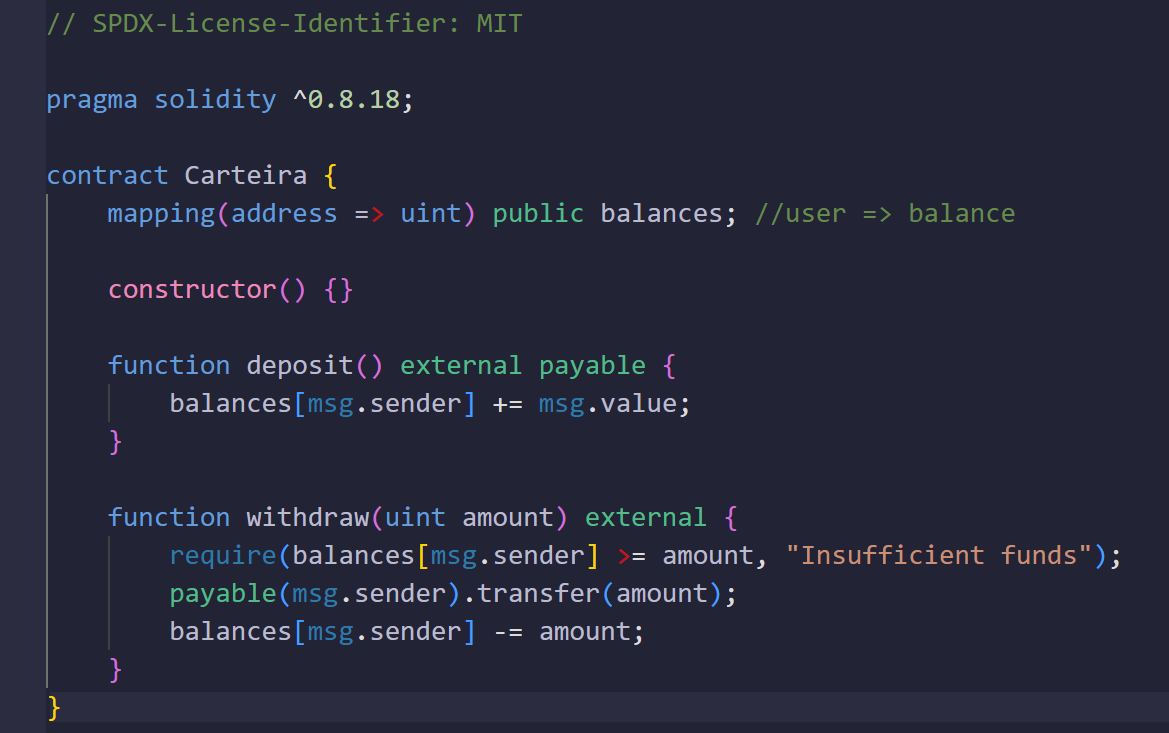
\includegraphics[width=0.5\linewidth]{figuras/VitimaRA.png}
    \caption{Contrato da Vítima}
    \label{fig:enter-label}
\end{figure}
\begin{figure}
    \centering
    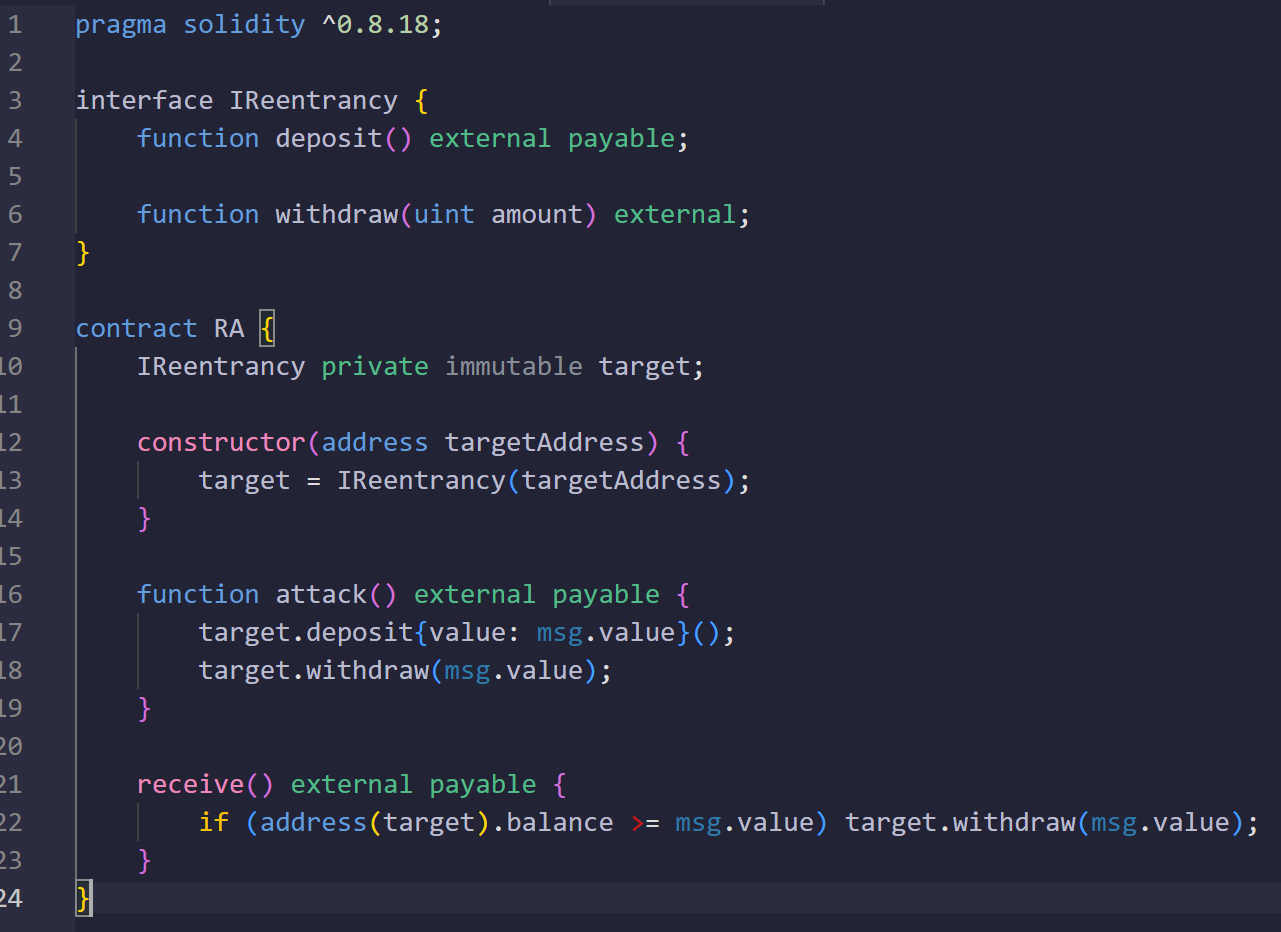
\includegraphics[width=0.5\linewidth]{figuras/RA.png}
    \caption{Contrato do Atacante}
    \label{fig:enter-label}
\end{figure}

Em um cenário hipotético, um invasor cria um smart contract, embora de forma mais sofisticada. O exemplo apresentado é simplificado, evitando a divulgação de ferramentas maliciosas. O contrato malicioso é então publicado na blockchain, identificando o endereço do contrato vulnerável.


Após o deploy do contrato malicioso, o atacante aciona a função "attack", realizando um depósito inicial no contrato alvo. Em seguida, ele invoca a função de saque do protocolo vítima, retirando a mesma quantidade recebida no depósito. Quando um smart contract recebe um saldo, a função nativa chamada "receive" é acionada. Embora, por padrão, essa função não execute ações, pode ser adaptada. No interior da função "receive", o invasor insere um código para realizar um novo saque, interrompendo a etapa de atualização do saldo do contrato vítima. Esse ajuste de balanço ocorre após o envio da transação, criando um loop até que o saldo do contrato seja exaurido. Em seguida, o invasor transfere o saldo final para outra conta, concluindo assim o ataque de reentrancy.

\textbf{Gas Griefing Attack \cite{GGA}:} Nos smart contracts de blockchain pública toda escrita é uma transação, e é exigido que toda transação pague uma taxa de gás -as taxas de gás sustentam a rede remunerando os validadores da rede-. 
Essa técnica consiste em fazer o contrato cobrar uma  taxa absurda ao ponto de zerar o saldo da carteira ou inviabilizar a lógica de negócio do contrato. 
Os contratos sucetiveis a esse ataque devem ser contratos que transferem dinheiro para outro endereço e disparam a função padrão receive, ou então em contratos que o atacante gostaria de interromper.
\begin{figure}
    \centering
    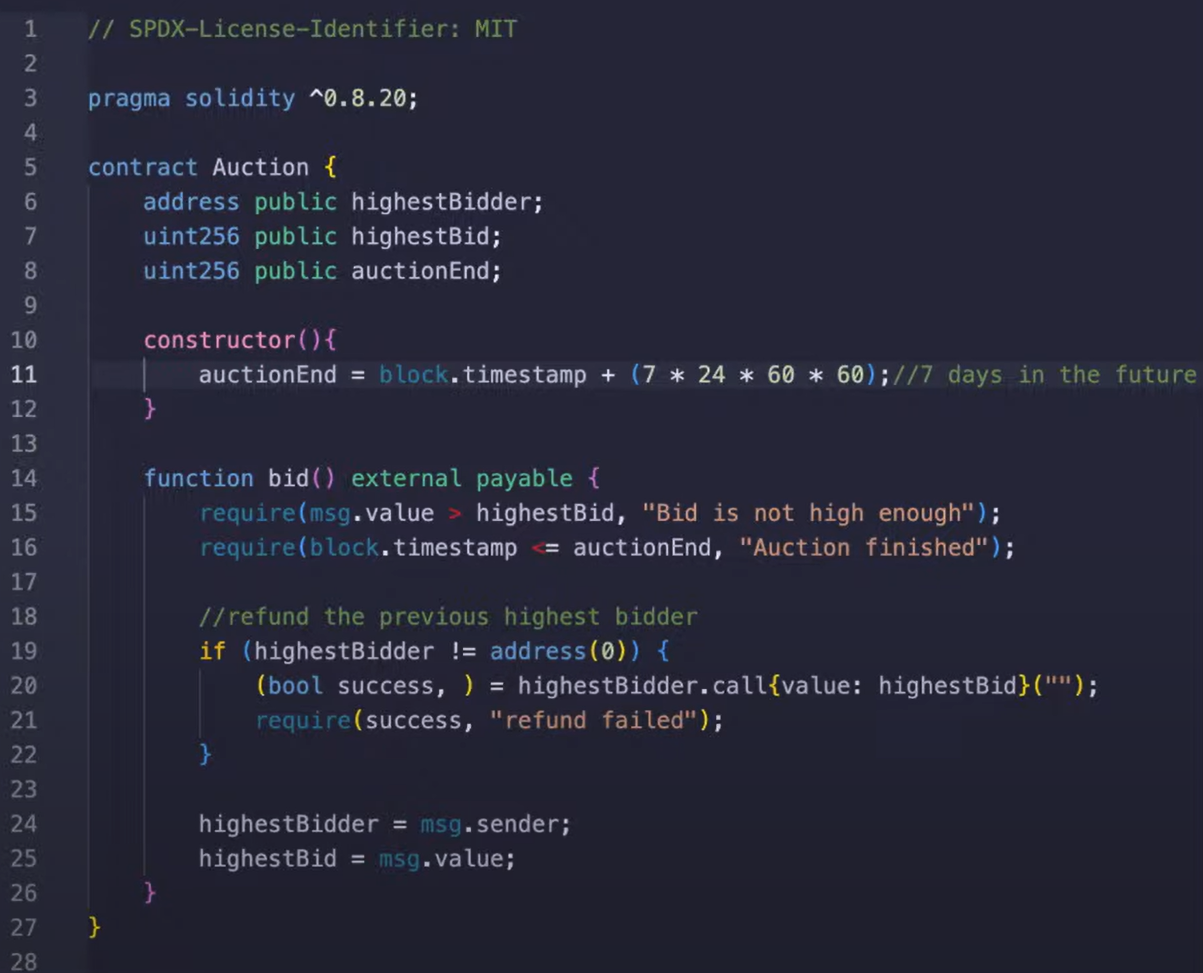
\includegraphics[width=0.5\linewidth]{figuras/Auction.png}
    \caption{Contrato de Leilão}
    \label{fig:enter-label}
\end{figure}

Este contrato de leilão foi concebido para operar ao longo de um período de 7 dias, apresentando uma função fundamental para dar lances. Quando um lance é submetido, o contrato realiza uma verificação para determinar se o novo lance supera o valor do lance máximo atual. Em caso afirmativo, ocorre uma atualização nas informações, resultando na alteração do vencedor do leilão para o usuário que ofereceu o novo lance. Além disso, os fundos são restituídos ao antigo vencedor do leilão.

Essa lógica de leilão busca promover a competição entre os participantes, garantindo que o usuário com o lance mais alto ocupe a posição de vencedor. A implementação de tal mecanismo proporciona dinamismo ao leilão, criando um ambiente em que os participantes podem ajustar seus lances para manter ou conquistar a liderança no decorrer dos 7 dias estabelecidos.

 \begin{figure}
    \centering
    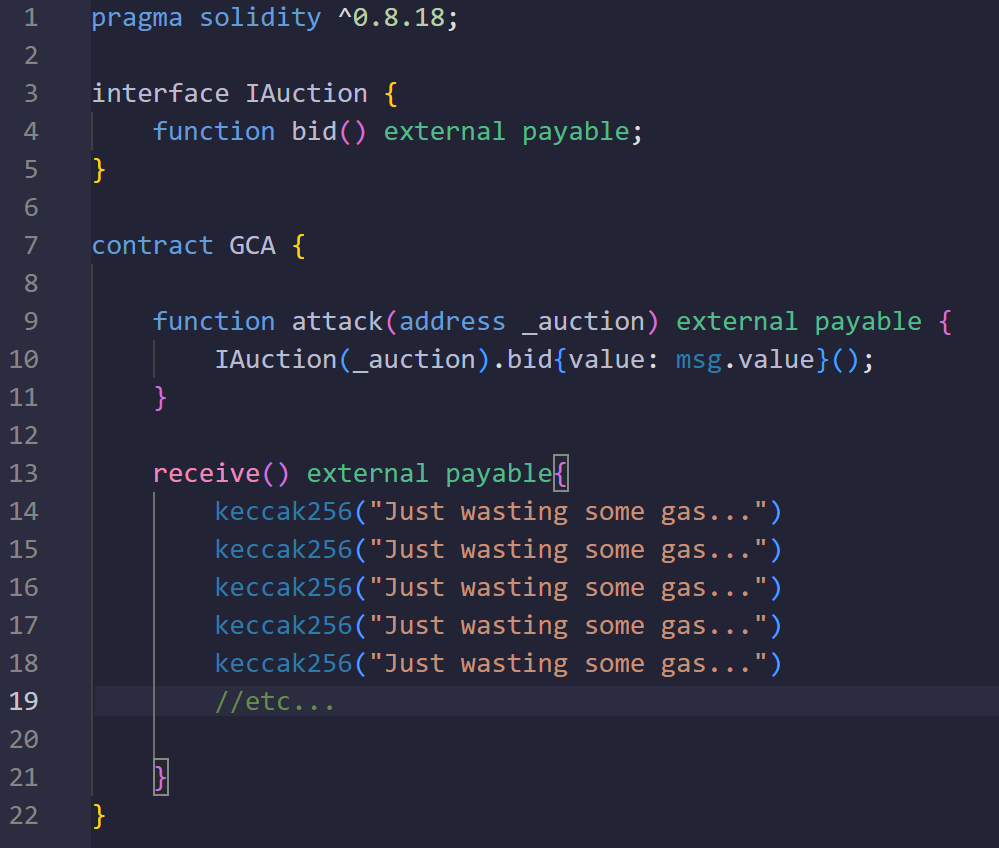
\includegraphics[width=0.5\linewidth]{figuras/GGA.png}
    \caption{Contrato do Atacante}
    \label{fig:enter-label}
\end{figure}

O contrato do atacante opera em consonância com o contrato do leilão, submetendo uma oferta superior à do atual líder. Quando outro participante oferece um lance superior ao do atacante, a função "receive" do contrato do atacante é invocada. Se o código presente em "receive"  for extenso ou complexo, isso pode acarretar em aumento das taxas devido à alocação de memória, podendo até ultrapassar o limite permitido para uma transação.

Quando um desses dois obstáculos ocorre, o contrato inteligente entra em um estado de erro, revertendo a transação original e mantendo o atacante como vencedor do leilão. Importante notar que o usuário que acionou a função enfrentará a perda de uma considerável quantia de gás da carteira, e em alguns casos, todo o valor destinado ao pagamento das taxas de transação.

Essa estratégia revela não apenas a manipulação do resultado do leilão pelo atacante, mas também destaca o potencial impacto financeiro adverso para quem efetuou a chamada da função. É crucial, portanto, que desenvolvedores e usuários estejam cientes dessas dinâmicas ao interagir com contratos inteligentes, priorizando a segurança e compreendendo as possíveis ramificações econômicas de suas ações na blockchain.

\section{Gerenciamento de Risco em Contratos Inteligentes}



\subsection{Práticas Recomendadas para Mitigação de Riscos}

\textbf{Reentrancy Attack \cite{RA}: }Sabendo a forma que um reentracy attack básico funciona, vamos ver duas principais observações que devem ser feitas para não cair em um ataque desse tipo.
\begin{figure}
    \centering
    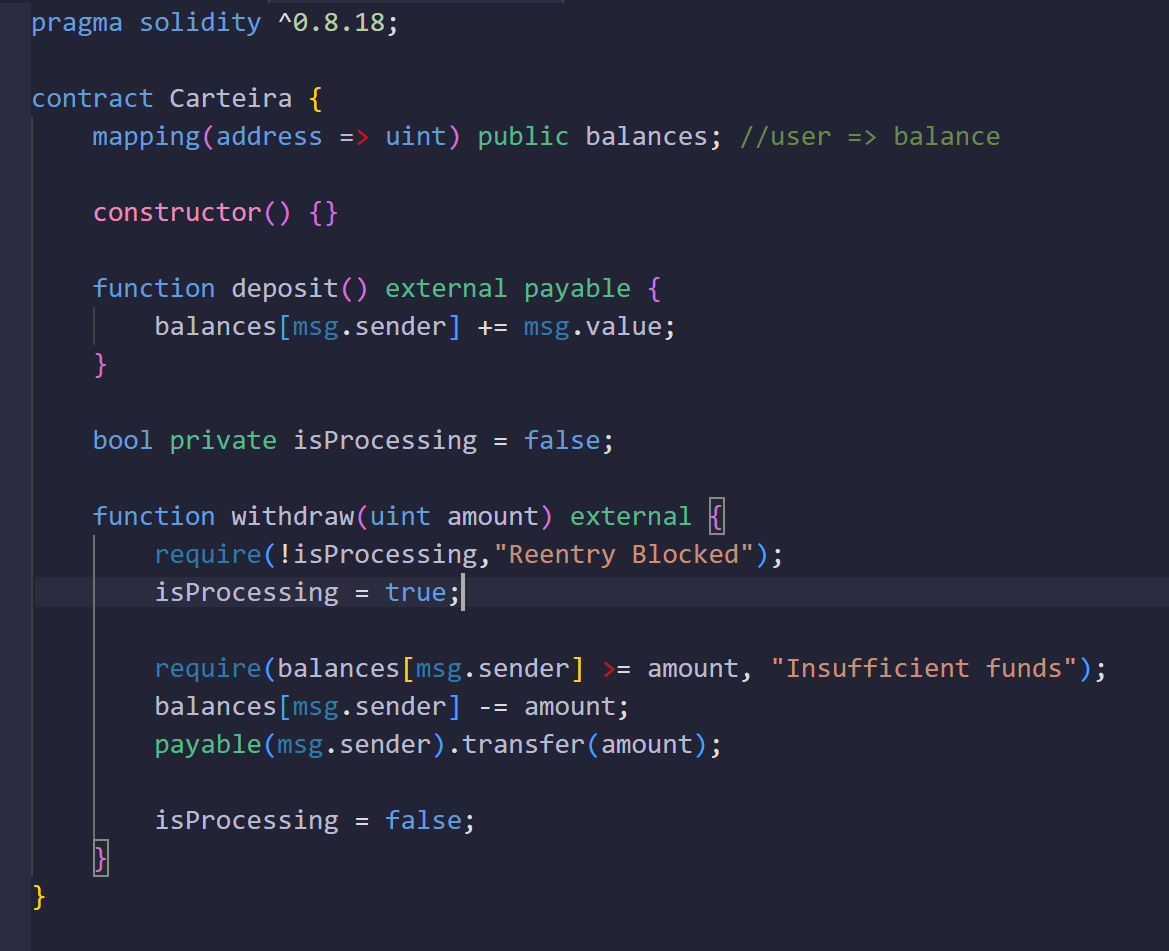
\includegraphics[width=0.5\linewidth]{figuras/RASolution.png}
    \caption{Solução Reentrancy}
    \label{fig:enter-label}
\end{figure}

É imperativo sempre manter a ordem das operações, dando prioridade à execução da atualização do saldo antes de qualquer transferência na função de saque. Ao organizar as etapas dessa maneira, evita-se a vulnerabilidade do código a ataques de reentrada com loops infinitos.

Outra medida eficaz para prevenir tais ataques na função de saque é a implementação de uma variável de controle dedicada. Essa abordagem, embora simples, proporciona uma camada adicional de segurança e pode ser aprimorada para uma implementação mais robusta. A lógica consiste em verificar e bloquear a possibilidade de reentrância na função de saque, impedindo potenciais explorações maliciosas.

Essas práticas, quando incorporadas, contribuem significativamente para mitigar a maioria dos ataques de reentrada, fortalecendo a segurança do protocolo.
\newline
\newline

\textbf{Gas Griefing Attack \cite{GGA}: } Diferentemente de alguns outros ataques a contratos inteligentes, esse tipo de ataque não possui uma solução simples, tornando-se assim uma ameaça significativa.

Em um cenário ideal, uma solução seria a atualização das linguagens de programação de contratos inteligentes para barrar sistemas como loops infinitos nas máquinas que executam os códigos.

Uma proposta mais radical seria alterar completamente o fluxo do contrato inteligente. Em vez de devolver imediatamente o dinheiro dos usuários quando alguém ultrapassa a oferta do atacante, o contrato poderia ser modificado para realizar a devolução apenas após o término do leilão. Essa alteração preservaria a integridade do contrato diante de ataques de GGA. No entanto, vale observar que uma mudança dessa natureza impactaria significativamente a lógica do contrato, exigindo adaptações no código para manter a equidade do leilão.

Por exemplo, se o dinheiro não fosse devolvido imediatamente quando alguém fizesse uma oferta maior, seria necessário implementar uma funcionalidade para permitir que o usuário com o dinheiro retido fizesse um novo lance utilizando os fundos bloqueados. Essas considerações destacam a complexidade de encontrar soluções eficazes que equilibrem a segurança do contrato com a manutenção da funcionalidade esperada.

\textbf{Os autores do artigo \cite{SMPP}} propõem a utilização da ferramenta "\href{https://github.com/eth-sri/securify2}{Securify}" como uma abordagem abrangente para identificar e compreender os problemas relacionados aos contratos inteligentes. Neste contexto, mais de 18 mil contratos inteligentes foram submetidos a testes, evidenciando a extensão e a diversidade do escopo de análise. A metodologia empregada pela "\href{https://github.com/eth-sri/securify2}{Securify}" permite a identificação de vulnerabilidades, destacando se os contratos inteligentes estão suscetíveis às formas mais básicas de ataques nesse domínio.

Essa abordagem não apenas oferece uma visão holística sobre a segurança dos contratos inteligentes, mas também fornece uma avaliação prática e abrangente da resistência desses contratos a ameaças potenciais. Ao realizar testes em uma quantidade significativa de contratos, os autores visam contribuir para uma compreensão mais profunda e generalizada dos desafios de segurança enfrentados pelos contratos inteligentes na blockchain.

 










 





